ハードウェア部分の実装に関しては,全天球ビデオカメラ2つ,PC2台,及び
OmniEyeBall1台を用意すればよい.

一方,ソフトウェア部分の実装に関しては,いくつか準備の必要がある
要素が存在する.

まず,ビデオストリーミングの方法について考える必要がある.
UDP等を用いて映像情報の送受信を行う必要がある.しかし,フレーム落ちの
問題など,現在使用されているビデオ会議アプリケーションのような堅牢で
高速な通信を実現するためには,高度な技術と時間を要する.
そこで,映像送受信については,すでに利用されているビデオ会議アプリケーション
を用いることにした.

しかし,ただ映像を送受信していては,PC側の操作に合わせて映像を回転させる
といった処理が出来ない.PC側では全天球ビデオカメラの映像を加工した後に
送信を行う必要がある.あるいは,PC側で表示するUIにおいて,OmniEyeBall側の
全天周パノラマ映像をそのまま表示させるのではなく,やはりクリックした人物の
顔を正面に移動させるなどの必要がある.
ここで,加工した映像をキャプチャしてビデオ会議アプリケーションに
認識させる方法と,一方で,送信されてきた映像をキャプチャーして,
以下で説明する画像加工ライブラリで扱えるようにする方法を考えなければならない.

この両方を解決するために,今回は仮想ビデオカメラを用いる.
仮想ビデオカメラとは,OBS-virtual-cam\cite{7}やUnityCapture\cite{8}
等のような,特定のアプリケーションの映像をリアルタイムでキャプチャし,
その映像をあたかも接続したビデオカメラの映像のように扱えるものである.
これを用いることで,ビデオ会議アプリケーションや画像加工ライブラリ
が,加工済みの映像や送信されてきた映像をビデオカメラの映像として認識し,
ストリーミングや加工が出来るようになる.

\begin{figure}[tp]
  \centering
  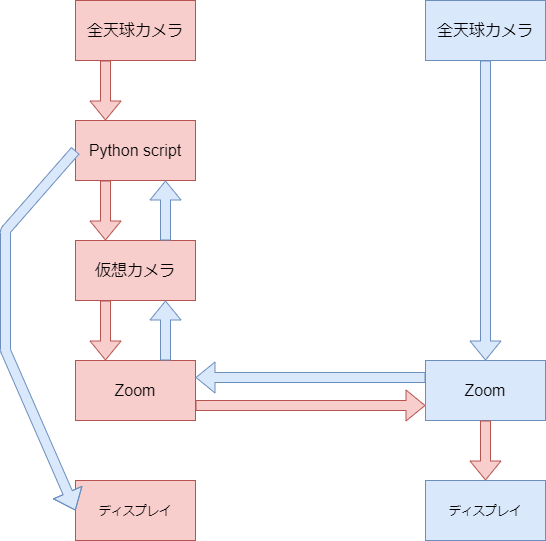
\includegraphics[scale=0.7]{fig/flow.png}
  \caption{映像の加工と送受信のフロー}
\end{figure}

次に,映像の加工方法について述べる.映像の加工はpythonなどで利用可能な
画像加工ライブラリを用いた.同時にPC画面に表示するUIもpythonのライブラリで作成した.

